\chapter{Machine Comprehension}
\label{chap:comprehension}
In this chapter a brief introduction to the machine comprehension task is given, followed by the application of our metric discussed in the previous chapter, that was defined for measuring similarity between concept graphs. After our baseline for the task presented.

The 2018 Semeval Task \textit{Machine comprehension using commonsense
	knowledge}\footnote{\url{https://competitions.codalab.org/competitions/17184}}
requires participants to train systems that can choose the
correct answer to simple multiple choice questions based on short
passages describing simple chains of events. Data for both training and
testing is extracted from the \texttt{MCScript} dataset
\cite{Ostermann:2018}. Some questions can only be
answered using commonsense knowledge, and are
explicitly labeled as such. For example, one passage might describe a
story of a gardener planting a tree, and one of the questions would
subsequently ask whether the gardener used his hands or a shovel to dig
a hole for the tree, even though the answer to this question is not
present in the passage. The top two systems, \texttt{HFL-RC}
\cite{Chen:2018} and
\texttt{Yuanfudao} \cite{Wang:2018} achieved accuracy scores of
$84.15\%$ and $83.95\%$ on the test data, respectively. In our experiments we used
semantic graphs to augment the \texttt{Yuanfudao} system, since its source
code is publicly
available\footnote{\url{https://github.com/intfloat/commonsense-rc}} and since it already employs successfully a
knowledge base representing semantic relationships among pairs of words.

\section{Comprehension, entailment, and knowledge bases}

In the next section we shall present a simple method for measuring
\textit{support}, the continuous counterpart of \textit{entailment},
based on graphical representations of meaning, and use this metric in a
baseline for machine comprehension and to improve a state of the art
MC system.
Although explicit representations of semantics are rarely used for this purpose,
in recent years there have been several attempts at leveraging lexical
ontologies in machine comprehension, and the approach of using textual
entailment as an intermediary task is also not new. \cite{Wang:2016}
achieves competitive results on the \texttt{MCTest} dataset
\cite{Richardson:2013} by generating
answer candidates and ranking them using a separate RTE system, which is
trained on the Stanford Natural Language Inference (SNLI) dataset
\cite{Bowman:2015}
but also relies on an explicit measure of lexical overlap between sentence
pairs. Other recent systems are various extensions of a baseline
proposed by \cite{Richardson:2013} that measures a weighted overlap
between pairs of bag-of-words representations, e.g. \cite{Wang:2015b}
applies the frame
semantic parser of \cite{Das:2010} and includes features representing
overlap between bag-of-frame and bag-of-argument representations.
Finally, the \texttt{Yuanfudao} system presented in the next chapter is the most
recent example of enhancing the performance of an MC system using a lexical
knowledge base: ablation studies show that their top-ranking accuracy score of
$83.84\%$ drops to $82.78\%$ if \texttt{ConceptNet}-based features are removed.

\subsection{Method}
\label{sec:method}

I used the metrics defined in the previous section.
Two (directed) edges are identical if their source
and target nodes and their labels are all identical. Based on early
findings we used only \textit{expanded} \texttt{4lang} graphs (see
Section~\ref{sec:4lang}) for measuring support. 
To create a simple baseline solution for the Machine Comprehension task,
I compare answer candidates to each question by comparing the degree of
support for each in the passage, based on the \texttt{4lang} representations of
each piece of text. For wh-questions we can create representations of
each answer by merging the question graph's wh-node with the graph of
each answer graph (see Figure~\ref{fig:merge}), for this I use the \textbf{/rally} endpoint of our service defined in the previous chapter. Our baseline method will simply pick the answer candidate with the higher support score.

\begin{figure}
	\centering
	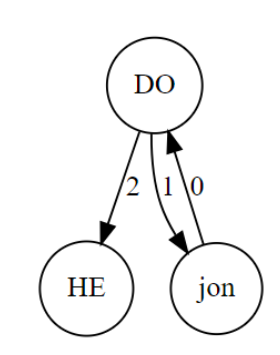
\includegraphics[scale=0.4]{figures/merge}
	\caption{Merged graph of answer candidate \textit{"Jon"} for the
		question \textit{Who did it?}}
	\label{fig:merge}
\end{figure}

\subsection{Experiments}
\label{sec:exp}

Demonstrating the algorithm behind my baseline, let's look at the example passage:
\begin{center}
	\textit{ "I went into my bedroom and flipped the light switch. Oh, I see that the ceiling lamp is not turning on. It must be that the light bulb needs replacement. I go through my closet and find a new light bulb that will fit this lamp and place it in my pocket. I also get my stepladder and place it under the lamp. I make sure the light switch is in the off position. I climb up the ladder and unscrew the old light bulb. I place the old bulb in my pocket and take out the new one. I then screw in the new bulb. I climb down the stepladder and place it back into the closet. I then throw out the old bulb into the recycling bin. I go back to my bedroom and turn on the light switch. I am happy to see that there is again light in my room."}
\end{center}
And a question related to the text: \textit{Which room did the light go out in?} and the answers:
\begin{itemize}
	\item \textit{"Kitchen."}
	\item \textit{"Bedroom."}
\end{itemize}
First the expanded graph from the text was built. After I constructed the merged graphs (for the demonstration, only the graphs without expansion was built) seen in Figure \ref{fig:merge1} and Figure \ref{fig:merge2}. The graph without merging can be seen in Figure \ref{fig:merge3}. After the merging, I compared both of the graphs to the passage graph applying my defined metric.

\begin{figure}
	\centering
	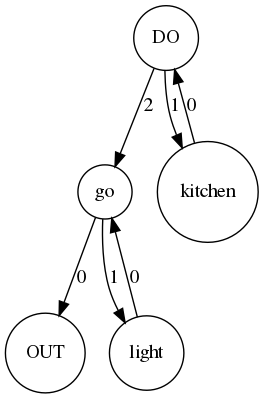
\includegraphics[scale=0.4]{figures/comp}
	\caption{Merged graph of answer candidate \textit{"Kitchen."}}
	\label{fig:merge1}
\end{figure}

\begin{figure}
	\centering
	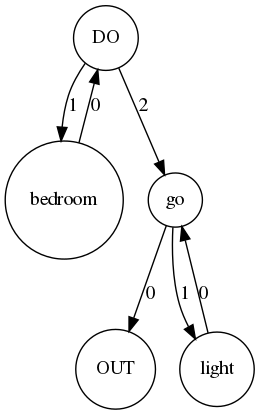
\includegraphics[scale=0.4]{figures/comp2}
	\caption{Merged graph of answer candidate \textit{"Bedroom."}}
	\label{fig:merge2}
\end{figure}

\begin{figure}
	\centering
	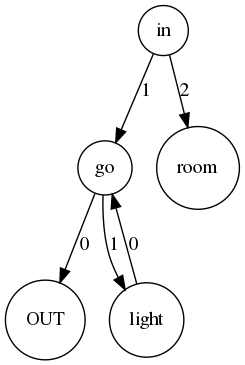
\includegraphics[scale=0.4]{figures/compdef}
	\caption{Graph built from the question}
	\label{fig:merge3}
\end{figure}

I tested the baseline method described in this section on a
subset of all questions in the train section of the MC dataset:
wh-questions that were not
categorized as "common-sense". Of this subset of 5,375 questions (of a
total of 9,731), our
method correctly answers 3,671, achieving an accuracy score of $68.3\%$.
I then proceeded to use the metric underlying our baseline as an
additional feature in the \texttt{Yuanfudao} system. 

In the next section I will briefly give an introduction into the field of deep learning in general, and particularly in NLP applications, and then I will demonstrate the Yuanfudao system.
%----------------------------------------------------------------------------
\section{Deep learning neural networks}
\label{sec:deep}

In this section I will introduce the basic deep learning related concepts necessary to understand the model described in the next section.

\subsection{Context}
With the recent increasing capabilities in computational power,
deep learning neural networks gained popularity again in recent years, after the AI winter ended. Since then neural networks became part of the everyday life, we hear about artificial intelligence being used in smart phones to enhance images quality or recognize certain settings and take a picture accordingly. AI is also being used in cancer research and other fields of bioinformatics, and personal assistants became extremely popular as well.

But even with the seemingly endless capabilities of artificial neural networks we are far from creating anything that could have the cognitive capacities of humans. This problem is considered by many to be AI-complete or AI-hard, meaning that creating a network that could keep up a human-like conversation would require data scientist and researchers to construct a universal artificial intelligence. A small but important step to achieve this is to create a system capable of doing simple reading comprehension tasks that also require some common sense knowledge.

The most common structures of these experimental neural networks include recurrent neural network layers and attention layers. Before the explanation of the function of these building-blocks, laying down the foundations is needed.

This section will introduce the essential deep learning mechanisms mainly used in NLP applications, and the main building blocks of the Yuanfudao system described in Section \ref{sec:yuanfudao}.

\subsection{Basics}
\begin{minipage}{\textwidth}
	Some arbitrary definitions this section uses:
	\begin{itemize}
		\item \textbf{Batch}: The chunks of training data that one iteration of the training uses. It's size can be a crucial parameter to set.
		\item \textbf{Epoch}: One training iteration is called an epoch. The number of epochs determines how long we want to train our network.
		\item \textbf{Learning rate}: \(\eta\) the velocity of the learning process. Setting it too low could result in slow learning and getting stuck in a local minimum, but setting it too high could result in jumping over the optimum and bouncing.
		\item \textbf{Accuracy}: The ratio of the correct predictions from all of the predictions. The goal of neural networks is to achieve high accuracy with on the test set.
		\item \textbf{Test set}: The part of the dataset that we don't use during the training of our neural network. This determines the actual accuracy of the network.
		\item \textbf{Training set}: The data that is used for training. The network is usually split into two parts with 80:20 ratio. We use the bigger set of data to train our network and we call this the training set.
		\item \textbf{Development set or Validation set}: The smaller portion of the data. We use this section to validate the network during its training. This section of the data shall not be used for training.
	\end{itemize}
\end{minipage}
\\
\\
People usually use supervised learning in the field of natural language processing to achieve the desired structure, but we might face multiple challenges while training. That's the reason why  optimization and regularization methods are needed.

\subsection{Optimization}
The goal of optimization is to overcome the following problems:
\begin{itemize}
	\item Local minimum
	\item Setting the learning rate
	\item Setting the batch size
\end{itemize}

We have touched on the first two briefly before, but setting the batch size is also very important. We give the training data to the network in batches, and we iterate through them multiple times (depending on the epoch).

Methods used for optimizing:
\begin{itemize}
	\item \textbf{Stochastic gradient descent}
	\item \textbf{Momentum}
	\item \textbf{Adaptive learning rate}
	\item \textbf{Adam} (Adaptive learning rate and momentum)
	\item \textbf{AdaMax} (Adam variant)
\end{itemize}

\paragraph*{Stochastic gradient descent}
\[g \leftarrow \frac{1}{batchSize}\Delta_w \sum_{i=1}^{batchSize}Loss(f_w(x_i), y_i)\]
Where f is the network itself.
\[w \leftarrow w - \eta g\]
This is a classical method for optimizing. It does not account for dynamic parameter settings. The system described in Section \ref{sec:yuanfudao} can use this function.
This is considered as our base, and only the differences between this and other optimization methods will be highlighted.

\paragraph*{Momentum}
\[g \leftarrow \alpha g + \frac{1}{batchSize}\Delta_w \sum_{i=1}^{batchSize}Loss(f_w(x_i), y_i)\]
Where \(\alpha\) is a parameter we can set.
This method has an added parameter, that helps taking into account the previous iterations, giving a momentum to the learning towards the optimum.

\paragraph*{Adaptive learning rate}
\[r \leftarrow r + g^2\]
Where r is a parameter that's initial value can be set.
\[w \leftarrow w - \frac{\eta}{\sqrt{r}} g\]
As the name suggests the adaptive learning rate uses a parametrization to slowly decrease the learning rate through time, depending on the previously calculated gradient.

\paragraph*{Adam}
\[r \leftarrow \varphi_r r + (1 - \varphi_r) g^2\]
\[s \leftarrow \varphi_s s + (1 - \varphi_s) g\]
Where s is a parameter that's initial value can be set and \(\varphi\) is a parameter of the decay rate.
\[w \leftarrow w - \frac{\eta s}{\sqrt{r}} g\]
Adam is one of the most popular optimizer function nowadays. It combines the adaptive learning rate and the momentum hence the name: Adam.

\paragraph*{AdaMax}
\[r \leftarrow \max(\varphi_r r, |g|)\]
\[s \leftarrow \varphi_s s + (1 - \varphi_s) g\]
\[w \leftarrow w - \frac{\eta}{1 - \varphi_s}\frac{s}{r}\]
A variant of the Adam optimizer. It was first described in the \textit{Adam: A method for stochastic optimization} article \cite{Kingma:2015}. It differs from Adam in that it uses a max operation and the infinity norm. The system described in Section \ref{sec:yuanfudao} can use this optimization function too.

\subsection{Regularization}
The goal of regularization is to avoid over-fitting. Over-fitting happens when our neural network produces good results on the training set's dedicated subset, the development or validation set, but it can't predict the expected outputs properly on a new dataset for example the test set. The network memorized the training set too much, and can function on that specific dataset only. It happens very often, so machine learning experts developed a couple functions to avoid this phenomenon.
\begin{itemize}
	\item \textbf{Weight decay}: Also known as L2 regularization. It uses a parameter to make sure that the previously learned weight won't influence the new one too much. \[w \leftarrow (1 - \eta \alpha)w - \eta \Delta_w Loss\]
	\item \textbf{L1 regularization}: This is a normalization method that modifies the cost function similarly to the L2 regularization. The difference is, that in this case the weights might get reduced to zero.
	\item \textbf{Dropout}: It randomly disables weights for an epoch, so they won't be used in that iteration.
	\item \textbf{Early stopping}: It stops the learning if the results on the development set haven't shown any progress in the last couple of epochs.
	\item \textbf{Noise injection}: It injects noise into the training set.
\end{itemize}

The system later described in Section \ref{sec:yuanfudao} uses dropouts while learning. This might cause the system's performance to fluctuate a little bit from epoch to epoch but it is a powerful tool for regularization and as we'll see later it manages to achieve consistently good results on the development set.

\subsection{Natural Language Processing with Deep learning}
As mentioned above the kind of layers used in Natural Language Processing are mostly recurrent neural network layers, attention layers and sometimes embedding layers.

\subsubsection{Embedding layers}

The function of embedding layers is to turn integer values to fixed length vectors, for example word embedding vectors discussed in Chapter \ref{chap:semanticparsing}. They are used mostly in natural language processing to work as word2vec translation.

When using embedding layers we want to find vectors for each word so that it can model the word's meaning. We achieve this by looking at the context the word usually appears in. If two words like \textit{apple} and \textit{orange} usually appear in the same context, than the vectors assigned to these words should have low cosine distance between them. It is explained in Chapter \ref{chap:semanticparsing}.

If you are building an NLP model, the embedding layer should be in the first layer, since its purpose is to make the transition from word to vector, and the word in this case is the input.

\begin{figure*}[!htb]
	\centering
	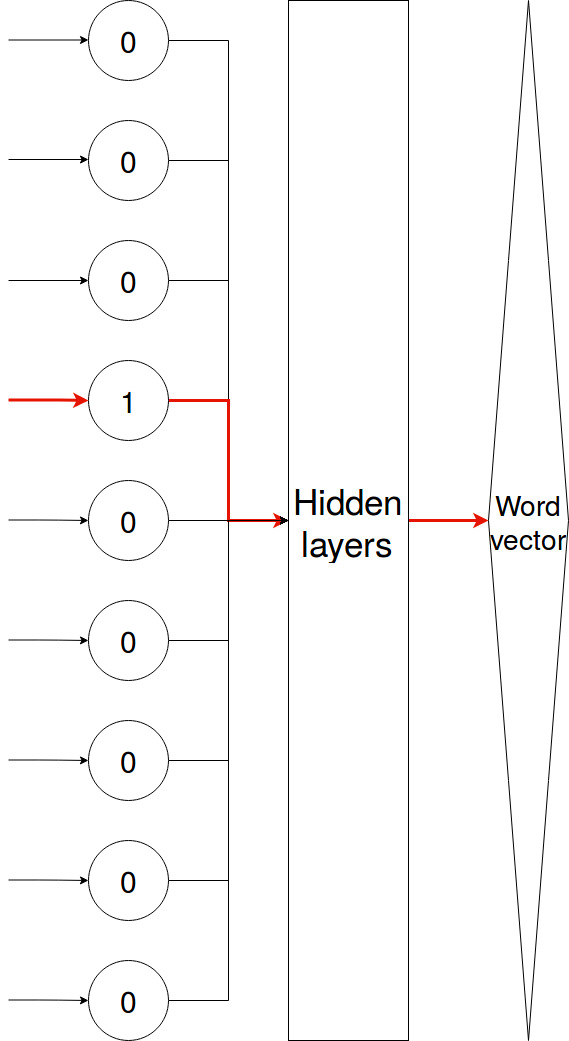
\includegraphics[scale=0.25]{figures/embedding_layer.jpg}
	\caption{An embedding layer.}
	\label{fig:embedding_layer}
\end{figure*}

The input dimension of this layer is the size of the vocabulary and the output dimension is the size of the dense vector. Usually the vocabulary size greatly exceeds the embedding dimension since the output vectors size is fixed and can range from 300 to 1000, and the vocabulary - depending on the dataset - can be way higher than that. See at Figure~\ref{fig:embedding_layer}.

They work mostly like a lookup table that can be trained. A lot of the times we use pretrained models, like the GloVe embeddings that have been trained on enormous datasets. We can also train them on our specific problem, or use the pretrained and our own embeddings simultaneously.
\FloatBarrier

\subsubsection{Recurrent Neural Networks}

In a simple feed forward neural network, the information only moves in one direction: from the input layer to the output layer. On the other hand recurrent neural networks take into account their immediate past, the output of the network with the previous timestamp. This internal "memory" like functionality allows the network to remember what it had calculated before. This is illustrated at Figure~\ref{fig:recurrent_net}.

At every timestamp the network gets two sets of inputs: the actual input at the timestamp and the hidden state of the network for the previous input. In one iteration it calculates its output using the calculated hidden state in the timestamp. It all could be imagined like the same feed forward network being repeated after one other.

The hidden state mentioned above is the "memory" of the network that is calculated with the previous hidden state and the input.

\begin{figure*}[!htb]
	\centering
	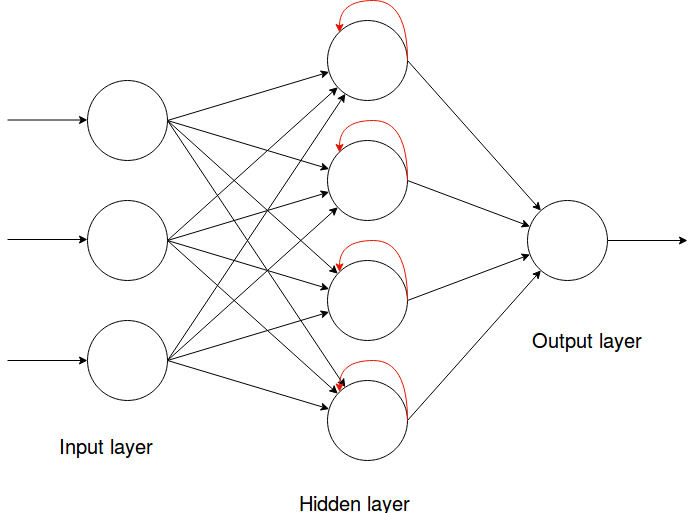
\includegraphics[scale=0.5]{figures/recurrent_neural_network.jpg}
	\caption{A recurrent neural network.}
	\label{fig:recurrent_net}
\end{figure*}

The backpropagation is also slightly different in this case, it's called backpropagation through time, you need to "unroll" the network (see at Figure~\ref{fig:unrolled}), and use the backpropagation starting from the right timestamps. Each timestamp's backpropagation could be understood as backpropagation on a separate feed forward neural network. 
\begin{figure*}[!htb]
	\centering
	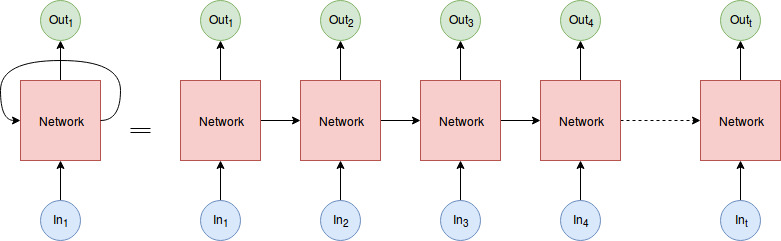
\includegraphics[scale=0.5]{figures/unrolled.jpg}
	\caption{Unrolled recurrent neural network.}
	\label{fig:unrolled}
\end{figure*}

The gradient vanishing or explosion can be a problem with this RNN.

There is a multitude of solutions for the exploding gradients, one of which is called gradient clipping. This is one of the method the state-of-the art system, Yuanfudao uses.

This technique is a very simple yet powerful way of dealing with exploding gradients. All it does is that it limits the size of the gradient, if its norm is higher than a set threshold.

RNNs can be used in supervised and also unsupervised learning. They are used when the data is sequential, like text, audio, etc.

\subsubsection{Long-Short Term Memory}
The system we worked with uses LSTM layers as its default RNN type.
Long-short term memory networks are the extension of the previously discussed recurrent neural network. The main difference is that it also has an internal long term memory. Usually these type of networks are more reluctant to have the exploding gradient problem.

Like the simple RNN, LSTMs also have hidden states, that are calculated slightly differently.
\\

\begin{minipage}{\textwidth}
	The LSTMs hidden states are calculated using three gates:
	\begin{itemize}
		\item \textbf{input gate}: determines whether to let new input in
		\item \textbf{forget gate}: determines whether to forget an input because it's not relevant anymore
		\item \textbf{output gate}: determines whether to let the input impact the output with the current timestamp
	\end{itemize}
\end{minipage}

These gates are analog and their values ranges from 0 to 1 with the sigmoid function. A simplified depiction can be seen at Figure~\ref{fig:lstm}\footnote{\url{https://en.wikipedia.org/wiki/Long_short-term_memory}}.
\begin{figure*}[!htb]
	\centering
	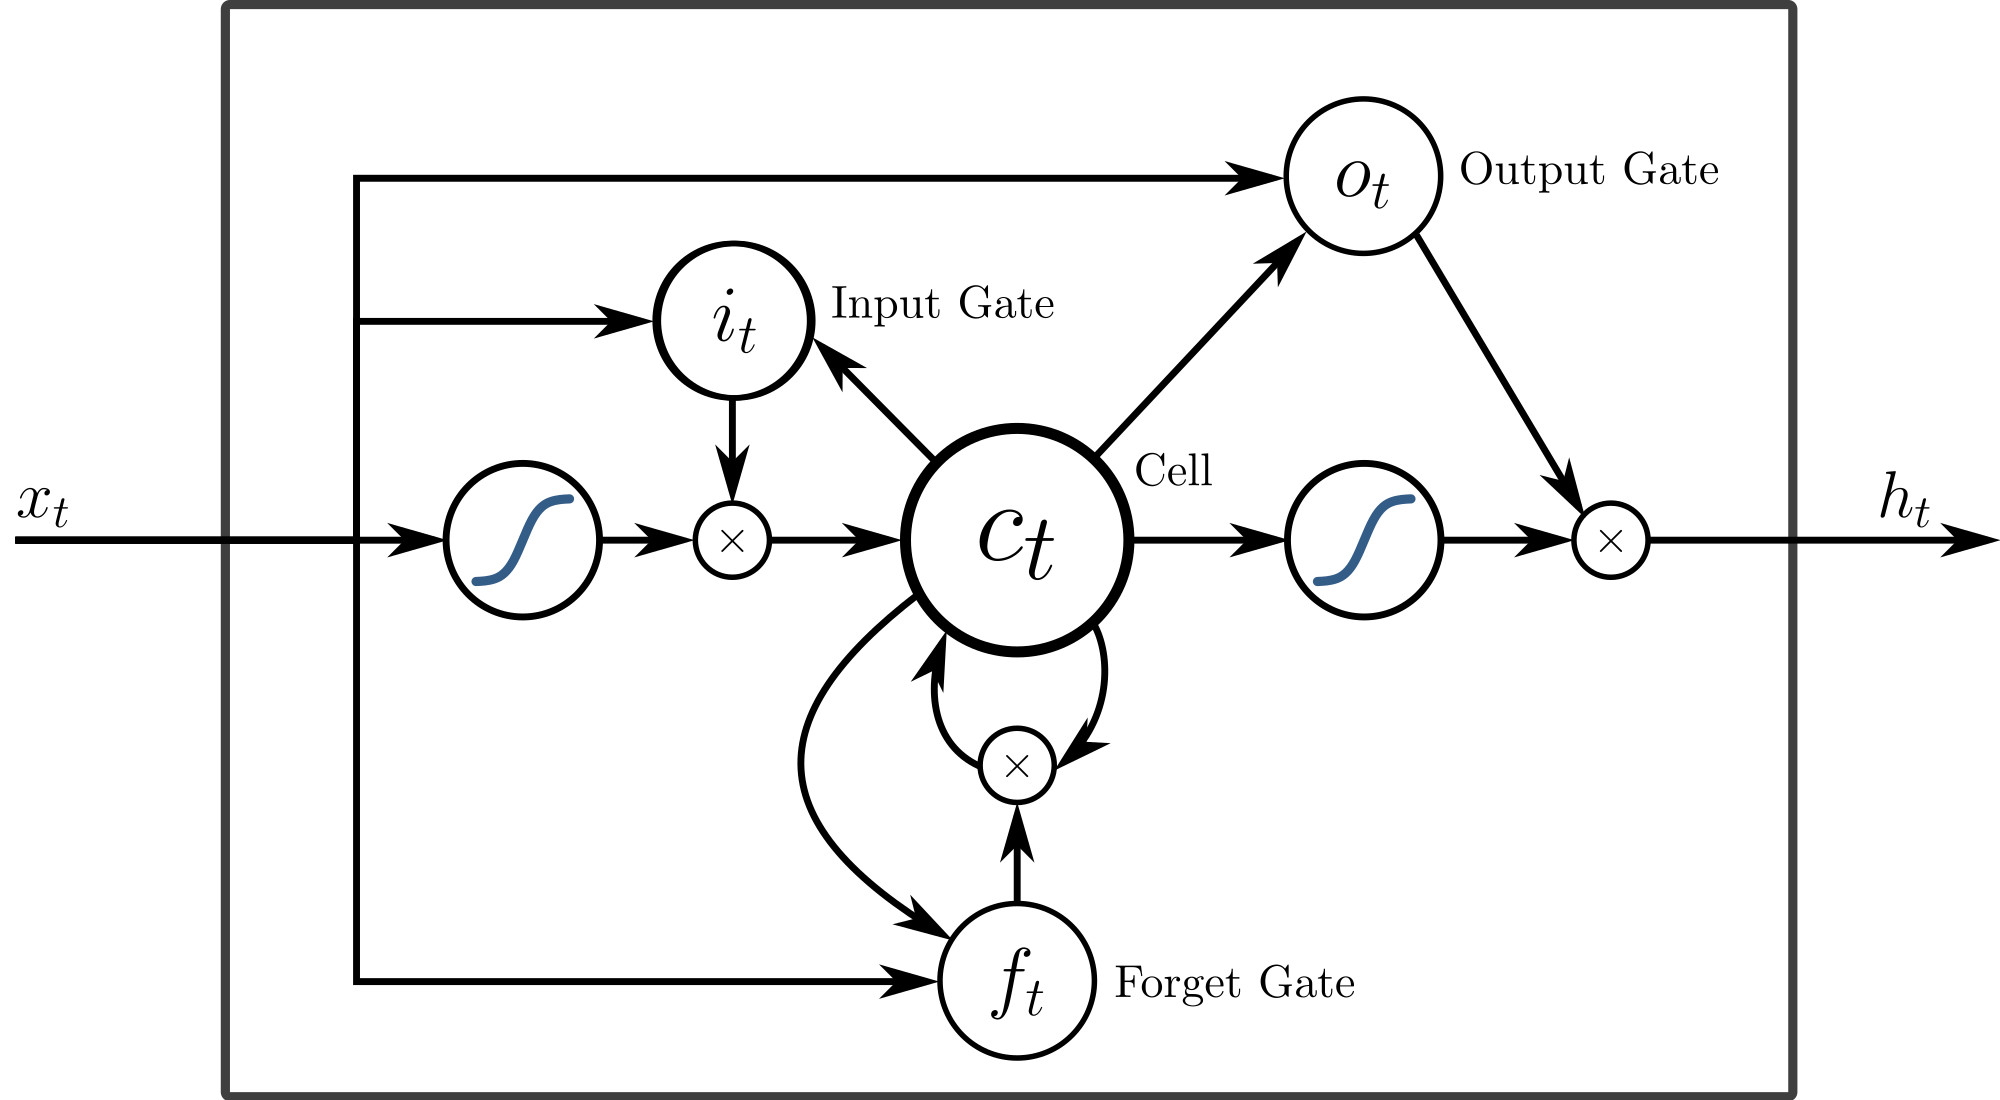
\includegraphics[scale=0.2]{figures/lstm.jpg}
	\caption{A long-short term memory network's gates.\\Image from Wikipedia}
	\label{fig:lstm}
\end{figure*}
\FloatBarrier

The sigmoid function allows this structure to be able to learn, meaning that we can use the backpropagation through time method described above.

Long-short term memory networks are used in natural language processing, but also in generative networks, like video or image description generation, text generation and so on.

\paragraph*{Bidirectional long-short term memory} also known as BiLSTM\\
BiLSTM networks are a variant of long-short term memory that read the input from the beginning to the end then also from the end to the beginning. The main idea behind this is that we may need not just the previous output, but also the next one too. These networks usually outperform simple LSTM systems in their predictions and the learning velocity too.

\subsubsection{Gated recurrent unit}
The system we worked with can use GRU layers as its RNN type, but it's not its default setting and it did not perform as good.
Gated recurrent units are also a type of RNN and have a similar structure (Figure~\ref{fig:gru}\footnote{\url{https://en.wikipedia.org/wiki/Gated_recurrent_unit}}) to the long-short term memory network, but has been shown to exhibit better performance on smaller datasets, than the LSTM.
\begin{figure*}[!htb]
	\centering
	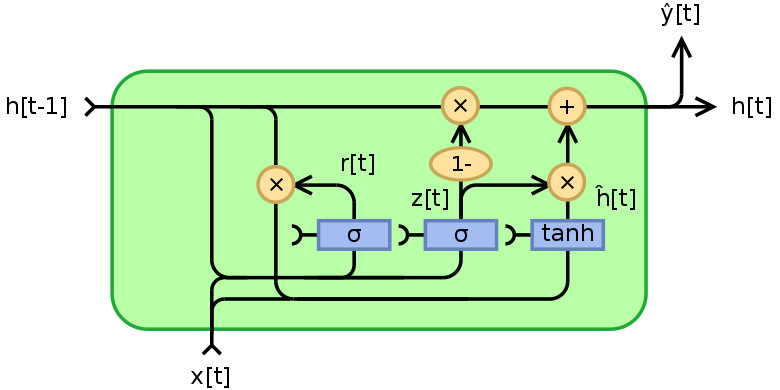
\includegraphics[scale=0.5]{figures/gru.jpg}
	\caption{A gated recurrent unit's gates.\\Image from Wikipedia}
	\label{fig:gru}
\end{figure*}

\begin{minipage}{\textwidth}
	It has four main building blocks:
	\begin{itemize}
		\item \textbf{update gate}: the gate gets the x[t] and the h[t-1] as its input and z[t] is the output on the image
		\item \textbf{reset gate}: the gate gets the x[t] and the h[t-1] as its input and r[t] is the output on the image
		\item \textbf{current memory content}: the gate gets the x[t], the h[t-1] and the r[t] as its input and \^{h}[t] is the output on the image
		\item \textbf{final memory at current time step}: the h[t] on the image
	\end{itemize}
\end{minipage}

Gated recurrent units are mostly used on the field of speech recognition and music modeling while the LSTM is more relevant on the field of natural language processing.

\subsubsection{Attention}
The Attention mechanism was first described in \cite{Bahdanau:2015} and was used for machine translation. Since then it became a widely used tool in natural language processing. The idea behind this mechanism is that when the neural network predicts the output, it only uses parts of the given input instead of the full input. That is where the most relevant information is concentrated and this mechanism only pays \textit{attention} to these parts and the network has to learn what to pay attention to.

Usually in the "sequence-to-sequence" tasks like MT there are two main parts of the model an encoder and a decoder. The encoder and the decoder are usually some type of RNN, mostly LSTM. The encoder is responsible for creating a so called context-vector from the input sequence. This context-vector has a fixed length and it serves as the representation of the sequence inside the model. The decoder then decodes this context-vector to a sequence again, in the case of the machine translation this sequence is in a different language. A depiction can be seen at Figure~\ref{fig:seq_to_seq}.
\begin{figure*}[!htb]
	\centering
	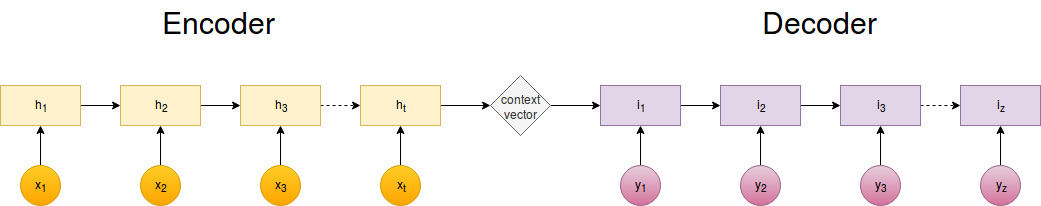
\includegraphics[scale=0.4]{figures/seq_to_seq.jpg}
	\caption{A sequence-to-sequence model with encoder and decoder.}
	\label{fig:seq_to_seq}
\end{figure*}

The attention mechanism described in \cite{Bahdanau:2015} was used in the decoder part of this model, the encoder functions the same way. The paper explicitly stated that this attention mechanism relieves the encoder from having to encode every sequence to a fixed length context vector. In this case we have a context vector for every word of the expected output. These context-vectors are the weighted sums of the encoder's states (\textit{annotations}).
\[c_i = \sum_{j=1}^{t} \alpha_ij h_j\]
Where \(\alpha\) parameter is calculated like the following:
\[\alpha_ij = \frac{exp(e_{ij})}{\sum_{k=1}^{t} e_{ik}} \]
and \(e_{ij}\) is its energy
\[e_{ij} = a(s_{i-i}, h_j)\]
This is an \textit{alignment model} that scores how well the input around \textit{j} and the output around \textit{i} match. This \textit{alignment model} is a feed forward neural network that is trained simultaneously with the other components of the system.
The decoder uses the previous state's output and its assigned context-vector when calculating its own target.
\[s_i = f(s_{i-1}, y_{i-1}, c_i)\]
The attention based model is at Figure~\ref{fig:attention}.
\begin{figure*}[!htb]
	\centering
	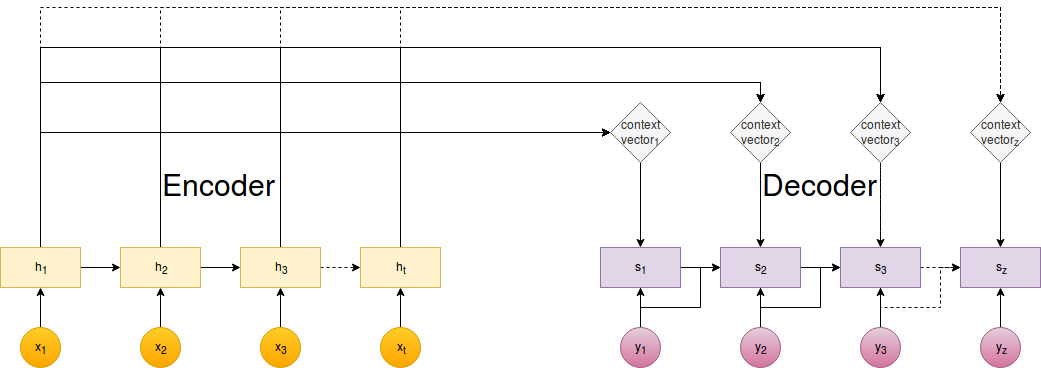
\includegraphics[scale=0.4]{figures/attention.jpg}
	\caption{A sequence-to-sequence model with encoder-decoder and attention.}
	\label{fig:attention}
\end{figure*}

A big advantage of using this mechanism is the ability to interpret our model. These days it's more important than ever to be able to tell why does the network predict what it predicts, and thanks to the attention mechanism we are able to say that (in a purely attention-based network). One example is shown at Figure~\ref{fig:interpretation}.

\begin{figure*}[!htb]
	\centering
	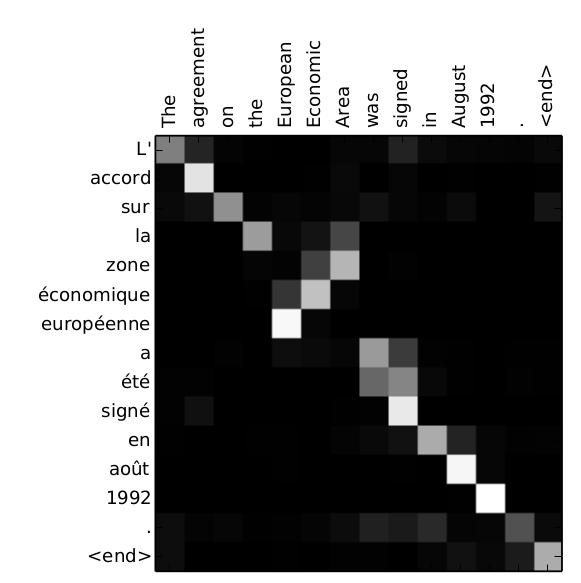
\includegraphics[scale=0.5]{figures/interpretation.jpg}
	\caption{An interpretation of a french - english sequence to sequence translation.\\Image from \cite{Bahdanau:2015}.}
	\label{fig:interpretation}
\end{figure*}

\begin{minipage}{\linewidth}
	Since its first description in \cite{Bahdanau:2015} the attention mechanism has been used for:
	\begin{itemize}
		\item \textbf{Image caption/description}: a convolutional neural network translates the image to the context vectors and the decoder creates a description for it. A recent system using attentions for image captioning is described in the \textit{Image Caption with Global-Local Attention} paper \cite{Li:2017c}.
		\item \textbf{Grammar representation}: in this case the decoder builds a grammatical representation for the input. On a related field there was a study regarding linguistic representations and attentions \cite{Kadar:2016}.
		\item \textbf{Advanced machine translation}: Since it was first introduced it has revolutionized the field of machine translation. A study on this field is \textit{Effective Approaches to Attention-based Neural Machine Translation} \cite{Luong:2015b}.
		\item \textbf{Machine comprehension tasks}: question answering based on a previously read text. The system described in Section \ref{sec:yuanfudao} is like this \cite{Wang:2018}.
	\end{itemize}
\end{minipage}
%----------------------------------------------------------------------------
\section{Yuanfudao system}
\label{sec:yuanfudao}
On the 2018 Semeval Task \textit{Machine comprehension using commonsense knowledge} competition the \texttt{Yuanfudao} \cite{Wang:2018} system reached second place with $83.95\%$ accuracy on the test data.

% Yuanfudao introduction
\subsection{The original system}

The \texttt{Yuanfudao} system implements a Three-way Attentive Network (TriAN), an ensemble of three LSTMs augmented with various attention mechanisms, to model for each question interactions between question, possible answers, and the passage that may or may not contain the correct answer to the question.

The system was implemented using python programming language and the \texttt{pytorch} package for the implementation of the neural network. The source code is available on Github\footnote{\url{https://github.com/intfloat/commonsense-rc}}.

% Yuanfudao preprocess

\subsection{Preprocessing}
This system processes the input data as follows:

\begin{enumerate}
	\item Using the \texttt{spacy} package's tokenizer function it generates the part of speech (pos) tag, named entity recognition (ner) tag and the lemma for each word in the passage, and the pos tags of the questions.
	\item It assigns a number representation and an offset for each word in the passage, questions and answers.
	\item It also saves the ids of the passages, questions and answers and whether the answer was correct.
	\item The preprocessor finds the words and lemmas in the questions and answers, that also occurred in the passage's word and lemma list. 
	\item It stores each word's frequency using the \texttt{wikiwords} library.
	\item It  establishes the \textit{ConceptNet} relation between the words of the passage and question and also between the words of the passage and answer.
	\item The preprocessor saves all this data to their respective json files.
\end{enumerate}


\paragraph*{Conceptnet} \cite{Speer:2017} \\

\textit{ConceptNet} plays a major part of the \texttt{Yuanfudao} system, as it was shown in the original paper \cite{Wang:2018}. This is a metric  used to show the possible relationship between two words. These relations could be "RelatedTo", "IsA", "Synonym", "PartOf" etc. 

The \textit{ConceptNet} itself is a large graph of general knowledge that has shown to be affective at determining word relations.

The preprocessor compares the words in the passage with the words in the "query" (question or answer) using \textit{ConceptNet} and stores only one of the matches per word, if there were any.

% System description

\subsection{System description}

An overview of the original system is reproduced in Figure~\ref{fig:dnn}.
\begin{figure}[h!]
	\centering
	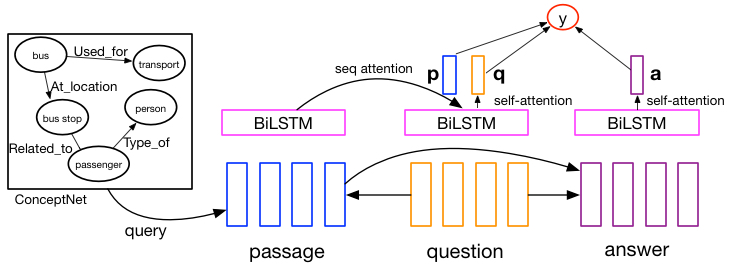
\includegraphics[scale=0.5]{figures/TriAN.jpg}
	\caption{Structure of the original network \cite{Wang:2018}}
	\label{fig:dnn}
\end{figure}

This system is a deep learning neural network consisting of embeddings, recurrent neural networks and attention mechanisms.

First the inputs generated in the preprocessing phase go through three embedding layers, each corresponding to the passage, question and answer respectively. There are also pos-embedding, ner-embedding and rel-embedding layers. The pos-embedding gets the passage's and the question's pos tags as its input, the ner-embedding layer gets the passage's ner-tags and the relation-embedding gets the relationship vectors generated using the \textit{ConceptNet}. This input embedding layer is shown in Figure~\ref{fig:embedding}.
\begin{figure}[h!]
	\centering
	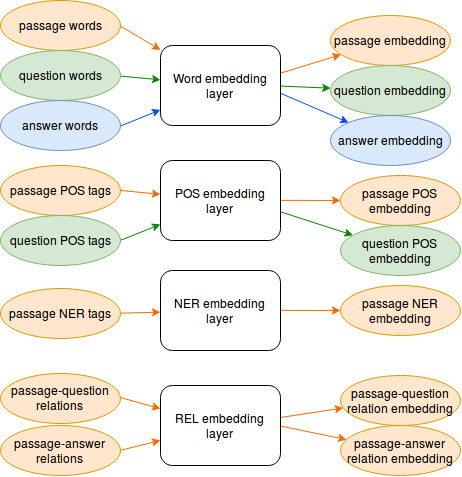
\includegraphics[scale=0.5]{figures/TriAN_embeddings.jpg}
	\caption{Structure of the input embedding layers.}
	\label{fig:embedding}
\end{figure}

The word embeddings' outputs are paired up (passage-question, answer-question, answer-passage) and go through a so called \textit{sequence attention matching layer}.
The sequence attention matching layer at its core uses the bmm function in \texttt{pytorch} which performs a batch matrix-matrix product of the input matrices.
This way it "matches" the two inputs together. This is shown in Figure~\ref{fig:attention_match}.
\begin{figure}[h!]
	\centering
	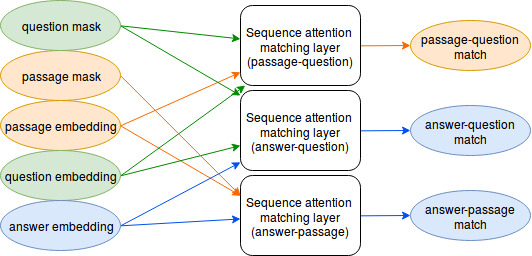
\includegraphics[scale=0.5]{figures/TriAN_attention_match.jpg}
	\caption{Structure of the \textit{sequence attention matching layers}.}
	\label{fig:attention_match}
\end{figure}

The system uses dropouts after the embedding and sequence attention matching layers to avoid over-fitting.

These layers are followed by three \textit{stacked bidirectional RNN layer}, each corresponding to the passage, question and answer respectively. It differs from the standard bidirectional RNN layer in one aspect: it can concatenate the hidden states of the RNN. By default the type of the RNN is LSTM, but it can also be GRU. Their inputs are sort of self explanatory. The passage's stacked bidirectional RNN layer gets the passage's word embedding layer, the output of the sequence attention matching layer for the passage-question input pair, the passage's pos- and ner-embedding layers, the word frequency tensor created with the \texttt{wikiword} library, and the two relation-embedding layer's output. The question's stacked bidirectional RNN layer expects the question's word and pos-embedding outputs on its input. The answer's stacked bidirectional RNN layer's inputs are the answer's word embedding output and  the output of the sequence attention matching layer for the answer-question and the answer-question input pairs. These RNN layers are shown in the Figure~\ref{fig:rnn}.
\begin{figure}[h!]
	\centering
	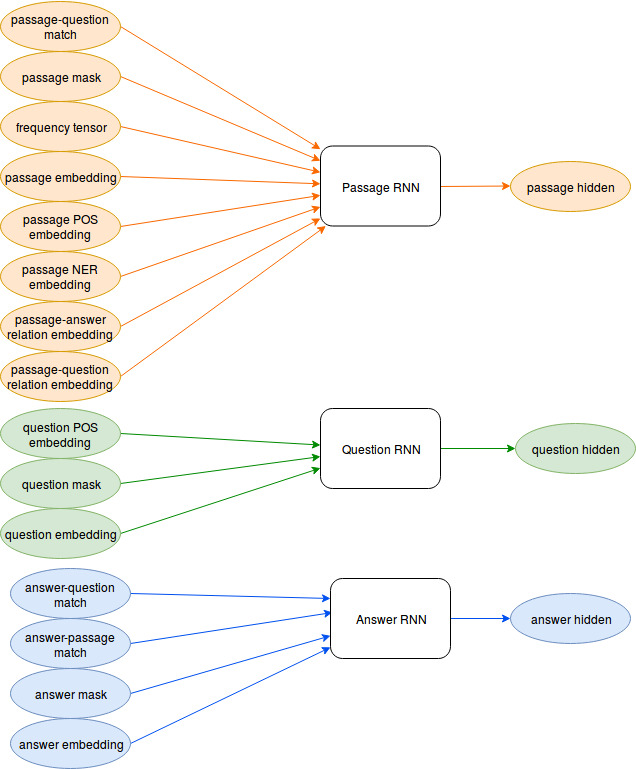
\includegraphics[scale=0.4]{figures/TriAN_rnn.jpg}
	\caption{Structure of the \textit{stacked bidirectional RNN layers}.}
	\label{fig:rnn}
\end{figure}
This layer implicitly uses a dropout rate for regularization.

The question's and the answer's stacked bidirectional RNN layer's outputs are used in two \textit{linear sequence attention layers}, or better known as \textit{self-attention layers over a sequence} for the question and the answer respectively. This layer is basically a linear layer slightly modified, so the infinite outputs are masked and it uses a softmax function at its output.

The passage's stacked bidirectional RNN layer's output is used differently. The system passes it and the question's \textit{stacked bidirectional RNN layer's} output to a \textit{bilinear sequence attention layer}, which is similarly to the sequence attention matching layer uses the bmm function as its core function.

The two linear sequence attention layer's and the bilinear sequence attention layer's output is passed through a weighted averaging function with their respective stacked bidirectional RNN layer's output. This part of the network is shown in Figure~\ref{fig:sequence_attention}.
\begin{figure}[h!]
	\centering
	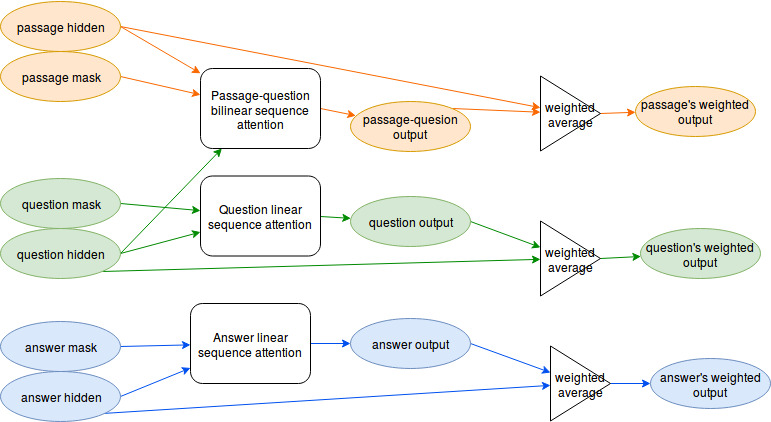
\includegraphics[scale=0.5]{figures/TriAN_sequence_attention.jpg}
	\caption{Structure of the sequence attention layer\\and the following weighted average function.}
	\label{fig:sequence_attention}
\end{figure}

The averaged passage output is passed through a \textit{linear feed forward layer} then multiplied by the answer's averaged output. The question's averaged output is passed through an other linear feed forward layer than multiplied by the answer's averaged output. At the end its all summed and sigmoid function used at its output. The output in this case is whether the answer was correct to the given question or not. This last section is at Figure~\ref{fig:output}.
\begin{figure}[!htb]
	\centering
	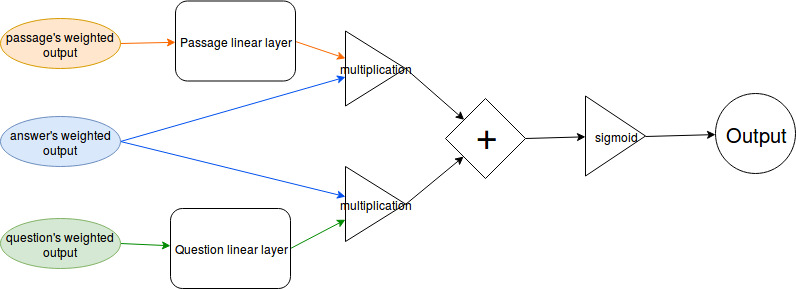
\includegraphics[scale=0.5]{figures/TriAN_output.jpg}
	\caption{Structure of the output of the network.}
	\label{fig:output}
\end{figure}


\subsection{Parameters}
\begin{minipage}{\textwidth}
	The \texttt{Yuanfudao} system has these following command line arguments:
	\begin{itemize}
		\item \textbf{GPU}: the training of the system can be done on GPU which is much faster than training it on CPU
		\item \textbf{using cuda}: \texttt{pytorch} can support CUDA for parallelization. The system uses CUDA by default.
		\item \textbf{optimizer}: the optimizer function can be adamax (default) or SGD
		\item \textbf{RNN type}: the RNN used by the system can be LSTM or GRU
		\item \textbf{dropout rate}: there are separate dropout rates for embeddings and RNNs
		\item \textbf{embedding dimension}: each embedding dimension in the system can be manually set
		\item \textbf{gradient clipping}: the gradient clipping threshold can be set
		\item \textbf{epoch}
		\item \textbf{learning rate}
		\item \textbf{batch size}
		\item \textbf{random seed}
		\item other parameters related to input handling, RNN settings and testing
	\end{itemize}
	You can read about the deep learning related arguments and their functions in Section \ref{sec:deep}.
\end{minipage}

\subsection{Learning curve}
\begin{minipage}{\linewidth}
	Without the recommended pretraining (Figure~\ref{fig:learning_curve}):
	\begin{itemize}
		\item Max dev accuracy: $82.7\%$ reached in the 26th epoch
		\item Train accuracy: $97.7\%$ reached in the 26th epoch
		\item Max train accuracy: $99.8\%$ reached in the 50th epoch
		\item Last dev accuracy: $81.9\%$
		\item Average dev accuracy after ten epochs: $81.9\%$
	\end{itemize}
\end{minipage}
\begin{figure}[!htb]
	\centering
	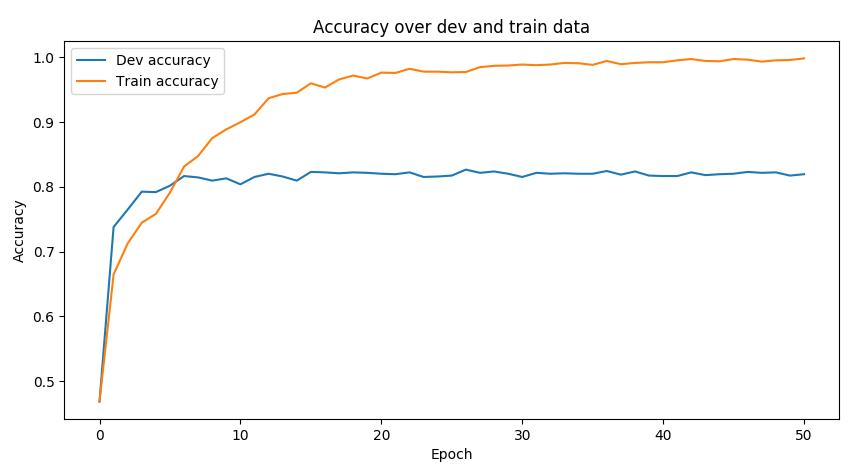
\includegraphics[scale=0.5]{figures/learning_curve.jpg}
	\caption{Learning curve without pretraining.}
	\label{fig:learning_curve}
\end{figure}

\begin{minipage}{\linewidth}
	With the recommended pretraining(Figure~\ref{fig:learning_curve2}):
	\begin{itemize}
		\item Max dev accuracy: $82.5\%$ reached in the 38th epoch
		\item Train accuracy: $99\%$ reached in the 38th epoch
		\item Max train accuracy: $99.7\%$ reached in the 50th epoch
		\item Last dev accuracy: $82.2\%$
		\item Average dev accuracy after ten epochs: $81.9\%$
	\end{itemize}
\end{minipage}
\begin{figure}[!htb]
	\centering
	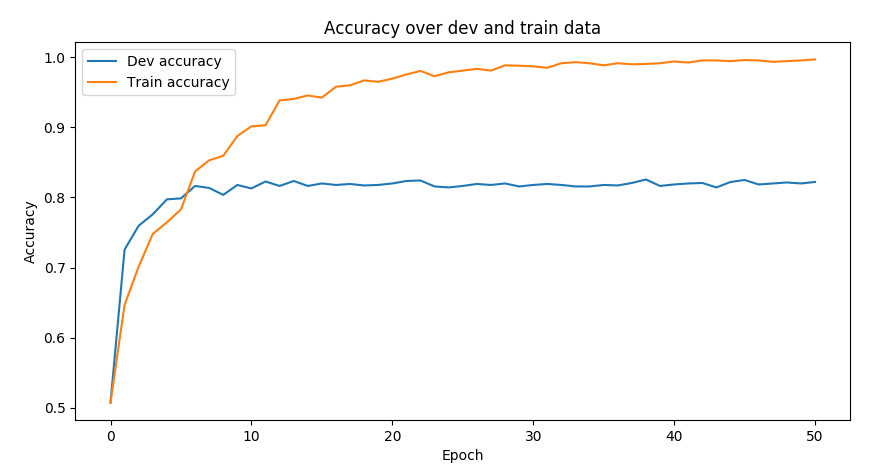
\includegraphics[scale=0.5]{figures/learning_curve2.jpg}
	\caption{Learning curve with pretraining.}
	\label{fig:learning_curve2}
\end{figure}

As you can see there is no significant difference between the learning curve with or without pretraining.

\section{Modifications}
Our modifications are available on Github\footnote{\url{https://github.com/GKingA/commonsense-rc}}.

We modified the preprocessing part of the system to incorporate the similarity calculating method from Chapter ~\ref{chap:comprehension}. The most straightforward way of incorporating our metric into the system is by creating vectors similar to those representing \textit{ConceptNet} relations between words of a passage and words in each answer candidate. Since these vectors represent
word-to-word relationships, we measure the support between pairs of \texttt{4lang} definition graphs, and for each word in the passage we take the maximum support score over all words of the answer candidate. Elements of a vector for a passage $P$ and a possible answer $A$ are hence defined as:

\[S^{(P, A)}_i = \max_{A_j \in A} S(P_i, A_j)\]

Elements of a vector for a passage $P$ and a question $Q$ are defined as:

\[S^{(P, Q)}_i = \max_{Q_j \in Q} S(P_i, Q_j)\]

Elements of a vector for a question $Q$ and an answer $A$ are defined as:

\[S^{(Q, A)}_i = \max_{A_j \in A} S(Q_i, A_j)\]

We used these new input vectors as the input of a new \texttt{4lang} embedding layer that functions similarly to the other embedding layers. It is shown at Figure~\ref{fig:4lang_embedding}. The input of this layer is 101 dimensional, since the similarities are on a scale to 0 to 100.

\begin{figure}[h!]
	\centering
	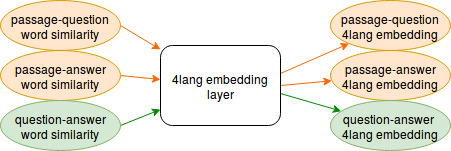
\includegraphics[scale=0.5]{figures/4lang_embedding.jpg}
	\caption{\texttt{4lang} embedding layer.}
	\label{fig:4lang_embedding}
\end{figure}

The outputs of this layer are passed to the RNN layers. This is depicted at Figure~\ref{fig:rnn_4lang}.

\begin{figure}[h!]
	\centering
	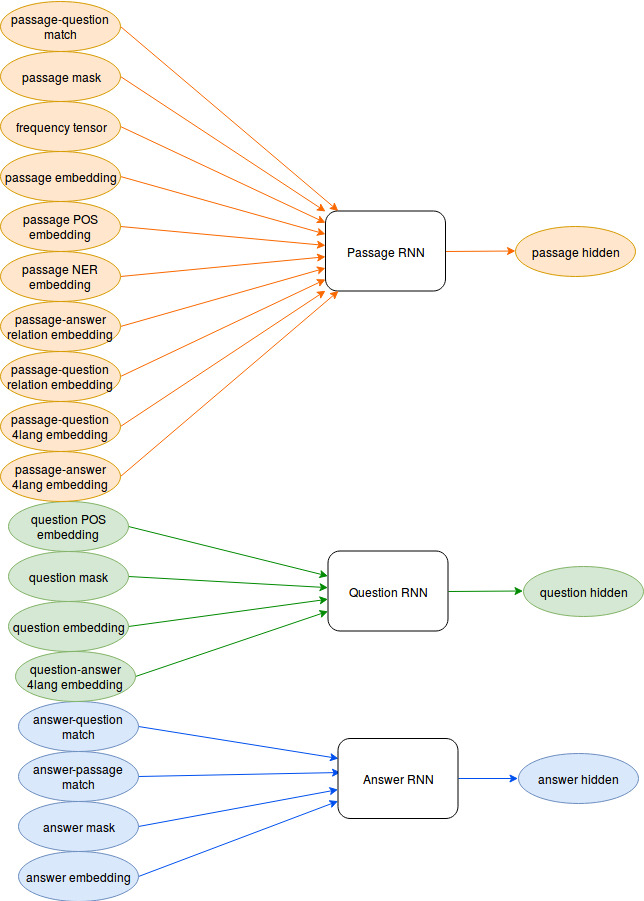
\includegraphics[scale=0.4]{figures/TriAN_rnn_with_4lang.jpg}
	\caption{Structure of the modified \textit{stacked bidirectional RNN layers}.}
	\label{fig:rnn_4lang}
\end{figure}

Since we also wanted to see how the system changes if we replace \textit{ConceptNet} relations with our metric, we also trained systems without \textit{ConceptNet} rel-embeddings.

\FloatBarrier

\section{The results}
The original \texttt{Yuanfudao} \cite{Wang:2018} publication said its system was able to reach $83.95\%$ accuracy on the test data. We were only able to reproduce a $80.3\%$ accuracy on the test set and $82.5\%$ on the development set with the recommended pretraining on the \texttt{RACE} \cite{Lai:2017} dataset. We will take these results as our bases of the comparison.

We tested our model by turning on and off the usage of \textit{ConceptNet} and \texttt{4lang}. There were 4 combinations: using neither, just \textit{ConceptNet}, just \texttt{4lang} and both.

\begin{table}[h!]
	\centering
	\begin{tabular}{ | l | c | r | }
		\hline
		model & dev & test \\ \hline \hline
		pretrained TriAN, no ConceptNet & 83.7\% & 81.9\% \\ \hline
		pretrained TriAN, with ConceptNet & 82.5\% & 80.3\% \\ \hline
		pretrained TriAN, with 4lang & 84.2\% & 81.5\% \\ \hline
		\textbf{pretrained TriAN, with both} & \textbf{83.4\%} & \textbf{82.9\%} \\ \hline
		TriAN, no ConceptNet & 82.8\% & 80.2\% \\ \hline
		TriAN, with ConceptNet & 82.7\% & 80.5\% \\ \hline
		TriAN, with 4lang & 83.2\% & 80.9\% \\ \hline
		TriAN, with both & 83.1\% & 80.8\% \\ \hline
	\end{tabular}
	\caption{Effect of \texttt{4lang} and \texttt{ConceptNet} on results}
	\label{tabl:res}
\end{table}

It is evident that without pretraining the Yuanfudao system performs best if we use the relation scores calculated from \texttt{4lang} graphs instead of the \textit{ConceptNet} relationships.
After pretraining the network on the \texttt{RACE} dataset the results show that using both of the relation metric is the most beneficial.